\chapter{Lab 0}
\setcounter{TASignatures}{0}
\setcounter{AsideCounter}{0}

\section{Introduction}
    \vspace{0.1em}

    \textbf{In this lab you gain experience with:}
    \begin{enumerate}
        \item How to download project files to the PLC
        \item How to download applications to the HMI
        \item How to make online edits to the ladder program
        \item How to make offline edits to the ladder program
        \item How to toggle a bit
    \end{enumerate}
    
    \vspace{1em}
    \textbf{In this lab you will be exposed to:}
    \begin{enumerate}
        \item Ladder logic
        \item Logical OR and Logical AND
        \item Normally closed contact (XIO)
        \item Normally open contact (XIC)
        \item Output coil (OTE)
    \end{enumerate}
    
\subsection{How to get credit}
Each lab after this will require each student to submit the completed pre-lab before they are allowed to begin working on the lab. The \textbf{pre-lab must be submitted to the TA before beginning work on the lab}. If it is not complete then you will be required to complete the pre-lab before you are allowed to begin working on the lab.

In order to get credit for completing each part of this lab, \textbf{you must personally read and complete each portion of the lab and demonstrate the completion to the TA}. Each section has one or more signature slots that must be signed by the TA to confirm that the section was completed. Each section is worth equal credit. 

\subsection{20 minute grace period}
To receive full credit, the lab must be completed and demonstrated during the assigned lab time. However, if you cannot complete the lab within that time, you can complete and demonstrate the lab within the first 20 minutes of the subsequent lab time and still receive full credit. \textbf{If the lab is not completed within the assigned lab time and is not completed within the 20 minute grace period, then the lab is considered late}. If you submit the lab late, then there will be a 20\% deduction compounded weekly.


\subsection{Safety}

The PLCs and equipment in this lab use \textbf{120VAC and 24VDC}. The equipment is considered finger safe, which means that accidental contact with the electrical circuitry is \textit{unlikely}. However, there are small gaps around the connections to the PLC and other equipment which expose small portions of bare wires or bare metal from the bussbars. 
\\
\textbf{DO NOT TOUCH ANY BARE WIRES or METAL EXPOSED AROUND BUSSBARS! YOU WILL BE SHOCKED!}
\\

\subsection{Lab agreement}

The planning of a program is often a very social activity, however the actual writing of the code is always an individual pursuit. In this class it is very much the same. Students are welcome to verbally assist each other, but each person is required to write their own code and personally complete each lab. In this way each student will gain valuable experience with programming PLCs. 

\textbf{The undersigned person guarantees that any and all work demonstrated to the TA in regard to this lab is a result of their own work with no unauthorized help. Further, they acknowledge all course and safety information which has been given.}

\signatureSlot{Student (Print \& Sign)}


\section{Downloading to the PLC}

In this section you will download the Lab 0 project to the programmable logic controller (PLC). Be careful not to \textbf{mix up downloading and uploading}. Downloading is pushing code into the PLC. Uploading is pulling the code from the PLC into the computer. In this class you should \textbf{never upload}. 

The code that is in the PLC when you arrive to the lab is most likely not the code that you left in it from the previous lab. So, make sure that you save your lab progress to the lab drive or to a flash drive for safe keeping. 

This section serves as \textbf{general instructions for downloading to the PLC}. Refer to this lab manual in future labs if you forget how to download to the PLC.

\subsection{Get the lab files from iLearn}

In this lab you will often be working with a pre-made lab PLC and HMI file. As the semester progresses this will change. However, for the next several labs you will need to logon to ilearn and download the necessary lab files to the lab PC at the beginning of lab. Download all the files in the Lab0 ilearn folder under content now.

\subsection{Open Studio 5000}

Studio 5000 is the development environment used to modify Allen Bradley PLC ladder logic and download to the PLC. To open the program, click the windows icon in the bottom left and navigate to a folder called \textbf{Rockwell Software}. Open the folder and select \textbf{Studio 5000}. This will launch the software.

A splash screen like the one in \figureautorefname \ref{fig:SplashScreen} should appear. Select \textbf{Existing Project}. From the drop down that appears, select the option that says \textbf{Project File}. Navigate to the Lab PLC project that was downloaded from iLearn and select the file, then click \textbf{Open}.

\begin{figure}[h]
\centering
\textbf{Studio 5000 Splash Screen}\par \medskip
\frame{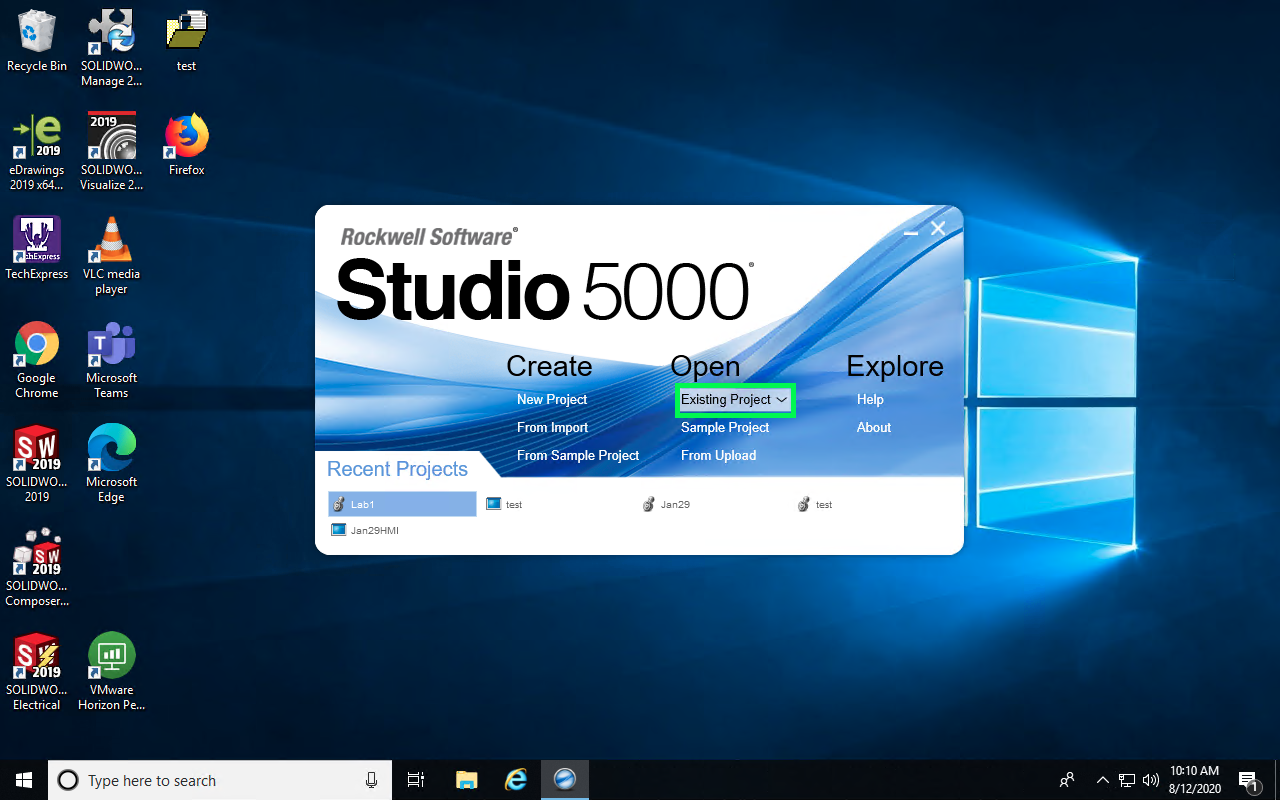
\includegraphics[width=3.2in]{Studio5000SplashScreen}}
\caption{Studio 5000}
\label{fig:SplashScreen}
\end{figure}

\subsection{Set the project path}

Now that Studio 5000 has been launched and the appropriate Lab project has been opened, you have to point Studio 5000 at the PLC which you will be using. This is referred to as setting the project path. \textbf{This is a very important step!}. Your classmates and TA will not be happy with you if you do not perform this step correctly, as it will cause you to \textbf{download to someone else's PLC}. 

\aside{Accidents happen and you will be forgiven for accidentally downloading to the wrong PLC. This happens to professionals as well. However, if the TA believes that you did this intentionally, \textbf{you may be asked to leave the lab}.}

\subsubsection{What is setting the project path?}
PLCs on a network are identified by their internet protocol (IP) address. The IP address for each of the PLCs in this lab corresponds with the lab seat number. Refer to \tableautorefname \ref{Table:PLCIpAddresses} to identify which PLC IP address corresponds with your seat number.

\textbf{Setting the project path is what Allen Bradley calls choosing the IP address of the PLC to which you will download code}.

\begin{table}[h]
\centering
\caption{PLC IP addresses}
\label{Table:PLCIpAddresses}
\begin{tabular}{c l | c l}
\toprule
Seat \# & IP Address & Seat \# & IP Address\\
\midrule
1 & $192.168.100.201$ & 2 & $192.168.100.202$ \\
3 & $192.168.100.203$ & 4 & $192.168.100.204$ \\
5 & $192.168.100.205$ & 6 & $192.168.100.206$ \\
7 & $192.168.100.207$ & 8 & $192.168.100.208$ \\
9 & $192.168.100.209$ & 10 & $192.168.100.210$ \\
11 & $192.168.100.211$ & 12 & $192.168.100.212$ \\
\bottomrule
\end{tabular}
\end{table}

\subsubsection{How do you set the project path?}

To set the project path, select the item in the menu bar called \textbf{Communications}. From the drop down, select \textbf{Who Active}. Here is where you will choose the PLC project path. Scroll to the PLC with the IP address associated with your seat and click the PLC to highlight it. Then select \textbf{Set Project Path}. 

\aside{If after highlighting the PLC, the option to set project path is still grayed out then you have either not selected the correct item or the project path is already pointing at your PLC. }

There is a plus icon beside the PLC that allows you to view items associated with that particular PLC. However, to set the project path you must select the outer most object. If this is confusing, refer to \figureautorefname \ref{fig:WhoActive}.


\begin{figure}[h]
\centering
\textbf{Who Active}\par \medskip
\frame{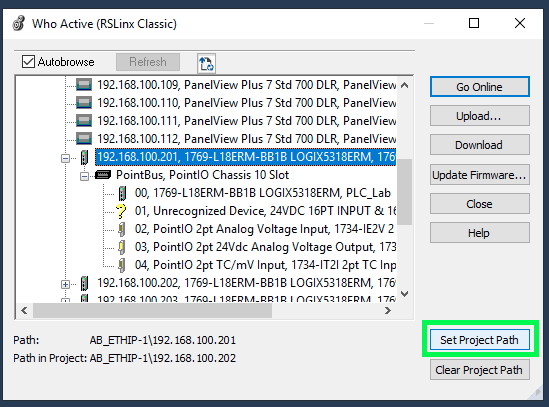
\includegraphics[width=3.2in]{WhoActive}}
\caption{Who Active}
\label{fig:WhoActive}
\end{figure}

\aside{In \figureautorefname \ref{fig:WhoActive} the user was sitting in seat number 1. \textbf{You most likely will not select the same PLC IP address shown in the image.} Refer to \tableautorefname \ref{Table:PLCIpAddresses} to verify which IP address is associated with your seat.}


\textbf{Do not select any other option other than Set Project Path!} After setting the project path, the option will be greyed out. Close the dialog window after setting the project path.

\subsection{Download to the PLC}
\label{subsection:DownloadPLC}

It is now time to download to the PLC. Again click the \textbf{Communications} option in the menu. From the dropdown, select \textbf{Download}. 

\aside{If the download option is grayed out, then you have either not set the project path or you are currently online with the PLC.} 

If you are online with the PLC, you will have to go to the Communications menu and select Go Offline before being able to Download.

\begin{figure}[h]
\centering
\textbf{Download Dialog}\par \medskip
\frame{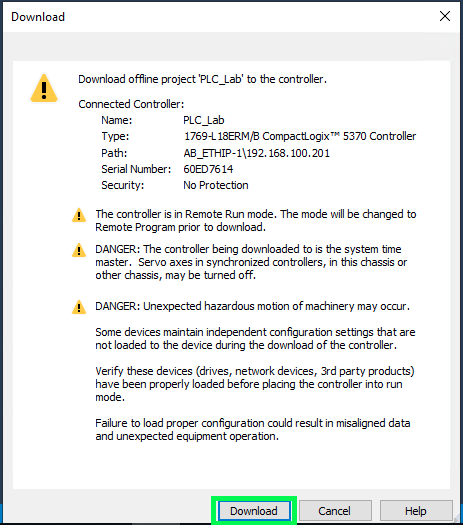
\includegraphics[width=3.2in]{DownloadMenu}}
\caption{Download dialog}
\label{fig:DownloadDialog}
\end{figure}

After selecting to download the code, a dialog window will appear. Click \textbf{Download} at the bottom of the dialog. For reference see \figureautorefname \ref{fig:DownloadDialog}.

\aside{In an industrial environment downloading can cause things to behave dangerously but in this lab environment we can ignore this warning.}

\aside{Before downloading the code to the PLC, Studio 5000 will automatically compile what you have written. If there is a compilation error, you will be informed and the download will be aborted.}


\subsection{Ensure that the PLC is in run mode}

After downloading the code to the PLC the code will not execute until the PLC is in run mode. Typically, after downloading to the PLC a dialog window will appear asking if you would like to return to run mode. Select, yes.

If for some reason the prompt does not appear, go to the Communications menu and select Go Online. Then go to the Communicaitons menu and select Run Mode.

\subsection{Open the Main Routine}

To view the code that is in the project, open the tasks dropdown in the left side menu. Here is where "routines" are kept. In each lab there will be a MainRoutine that houses the code. Refer to \figureautorefname \ref{fig:MainRoutine}. Double click the MainRoutine to open and view the code.

In \figureautorefname \ref{fig:TheCode} the code housed in MainRoutine is displayed. Notice there is a comment denoting the rung which you will be editing later in the lab. Also notice that the side bars of the "ladder" are green. This means that this code is currently "being scanned" or "being executed" by the PLC. If the PLC were not in run mode then the side bars would not be green. Also, if the user were not online with the PLC the side bars would not be green. 

\aside{The side bars being green is meant to signigy that they are energized. Ladder logic is intended to be read like an electrical schematic. Things that are green are energized. Notice that the \textbf{normally open contacts} associated with $Lab0.October$ and $Lab0.November$ are grey as is the \textbf{coil} associated with Lab0.Its\textunderscore Fall. This means that these are not energized.}

\begin{figure}[h]
\centering
\textbf{Tasks Dropdown}\par \medskip
\frame{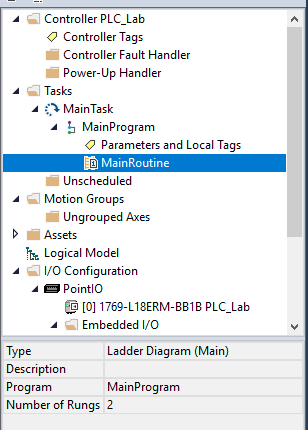
\includegraphics[width=3.2in]{MainRoutine}}
\caption{Tasks Dropdown and Main Routine}
\label{fig:MainRoutine}
\end{figure}


\begin{figure}[h]
\centering
\textbf{The Lab0 MainRoutine}\par \medskip
\frame{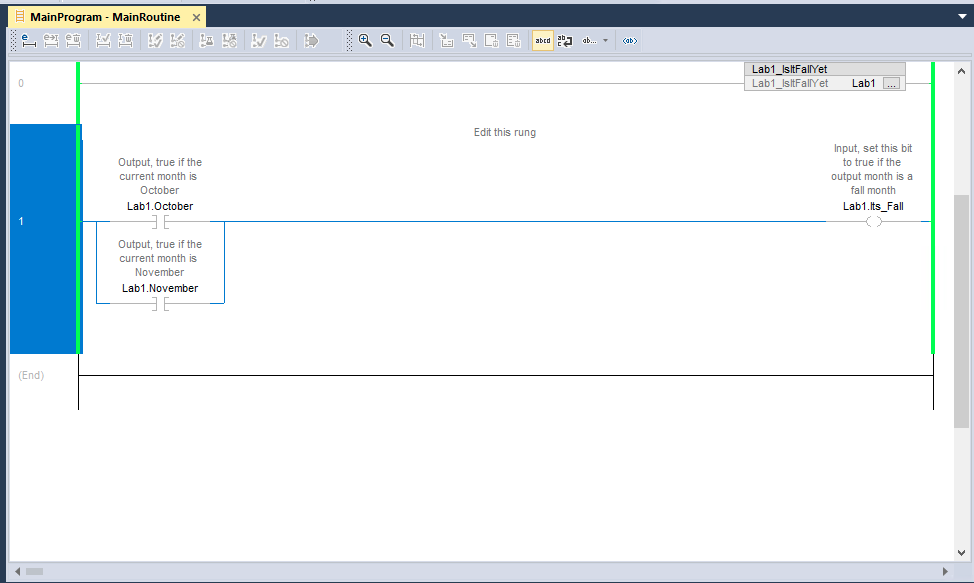
\includegraphics[width=3.2in]{Code}}
\caption{The code housed in the MainRoutine}
\label{fig:TheCode}
\end{figure}


\subsection{Go Online}
\label{subsection:GoOnline}

After downloading and ensuring that the PLC is in Run Mode, it is time to Go Online. Going online allows you to see the actual current state of the PLC and monitor the code as it executes. \textbf{Go to the communications menu and select Go Online}.

\aside{The code that is in Lab 0 is supposed to decide if it is Fall based on the month. However, you may notice that there is a logical error. We will fix this later on.}

\TASignatureSlot


\section{Downloading to the HMI}

PLCs work hand in hand with the human machine interface (HMI). The HMI is how operators are able to give input to and view the state of the machine. In this section you will learn how to restore an archived HMI application, generate a runtime application, and download the runtime application to the HMI.

\subsection{Open FactoryTalk View Studio}

The software used to edit HMI applications and download those applications to the HMI is called FactoryTalk View Studio. \textbf{Click the windows icon in the bottom left and navigate to FactoryTalk View Studio}. 

When the program launches, a dialog will appear asking if you would like to open an application or create a new application. The HMI files that we distribute cannot be opened through this dialog window. \textbf{Click cancel. This will close the dialog window}. 

\aside{To distribute HMI files they must be distributed as "backups". This is an odd idiosyncrasy of the FactoryTalk View Studio. These backups can't be opened through the initial dialog window. Rather, they must be "restored".}

\subsection{Restore the HMI application}

To restore the HMI application that you downloaded from iLearn, \textbf{go to the tools menu and select Application Manager}. This will open the FactoryTalk View ME Application Manager. This is actually a separate program that is launched. \textbf{Highlight the button beside Restore Application and click next}. 

You are then prompted for the location of the application archive. \textbf{Click the box with the three periods (ellipse) to open a file explorer windown}. Navigate to the application archive file downloaded from iLearn \textbf{open the file}. This will return you to the FactoryTalk View ME Application Manager Manager. \textbf{Click next}.

You are now prompted for a name to be given to the application. \textbf{Enter Lab0 and click finish}. 

\aside{You may be prompted to verify that you are ok with overwriting an existing HMI application with the same name. Be aware that if you have made changes to the HMI application and reopen the distributed archive file and overwrite your previous application, you may lose progress.}

\aside{Sometimes when you attempt to restore an application and give it a name that is already used, Factory talk will not be able to overwrite the other application. In this case, give the application a name which ends with your tech username. ie. Lab0\_jtroberts.}

After following all the above steps, the FactoryTalk View ME Application Manager will return to the initial screen. \textbf{Close the FactoryTalk View ME Application Manager}.

\subsection{Open the Restored Application}

Once the application archive file has been restored, the application can be opened. \textbf{Go to the file menu and select Open Application}. In the dialog that appears, \textbf{find and highlight the application name} that you have given to the application that was restored (should be Lab0). \textbf{Click open}.

\subsection{Communication Setup}

The HMI needs to be able to write and read information from the PLC. For this to be possible, the HMI will need to know the IP address of the PLC. 

To point the HMI at the PLC, on the left hand side menu \textbf{click the plus beside FactoryTalk linx}. Then \textbf{double click Communication Setup}. Refer to \figureautorefname \ref{fig:HMICommunicationSetup}.

\begin{figure}[h]
\centering
\textbf{HMI Communication Setup Location}\par \medskip
\frame{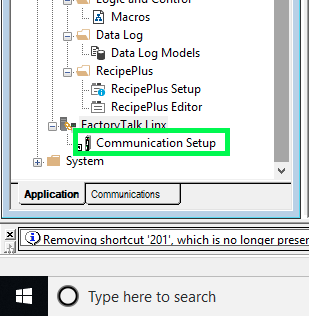
\includegraphics[width=3.2in]{CommunicationSetup}}
\caption{Where to find the HMI Communication Setup}
\label{fig:HMICommunicationSetup}
\end{figure}

In the window that opens, navigate to the PLC associated with your lab seat. \textbf{Click the plus beside the PLC associated with your lab seat}. \textbf{Click the plus beside the item named PointBus}. Now, \textbf{highlight the item 0}. Refer to \figureautorefname \ref{fig:PLCSelectionHMISetup} for clarification.

\aside{In \figureautorefname \ref{fig:PLCSelectionHMISetup} the user was sitting in seat number 1. \textbf{You most likely will not select the same PLC IP address shown in the image.} Refer to \tableautorefname \ref{Table:PLCIpAddresses} to verify which IP address is associated with your seat.}

\begin{figure}[h]
\centering
\textbf{Select the PLC in the HMI Software}\par \medskip
\frame{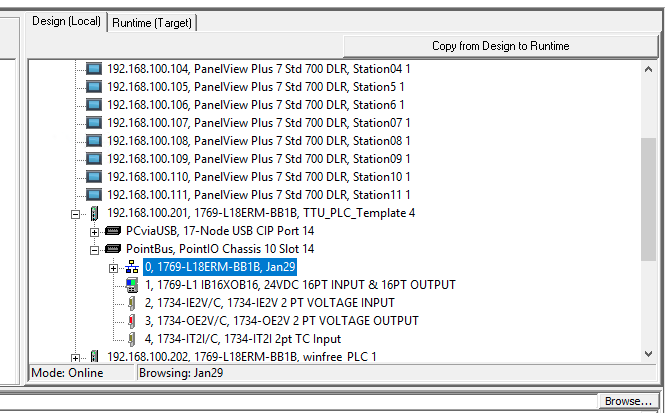
\includegraphics[width=3.2in]{SelectPLCinHMI}}
\caption{PLC Selection in HMI Communication Setup}
\label{fig:PLCSelectionHMISetup}
\end{figure}

With the correct PLC highlighted, \textbf{highlight PLC in the Device shortcuts to the left and click apply}. Next, \textbf{click copy from design to runtime}. Refer to \figureautorefname \ref{fig:CopyfromDesignToRuntime} to clarify.

\begin{figure}[h]
\centering
\textbf{Copy from design to runtime}\par \medskip
\frame{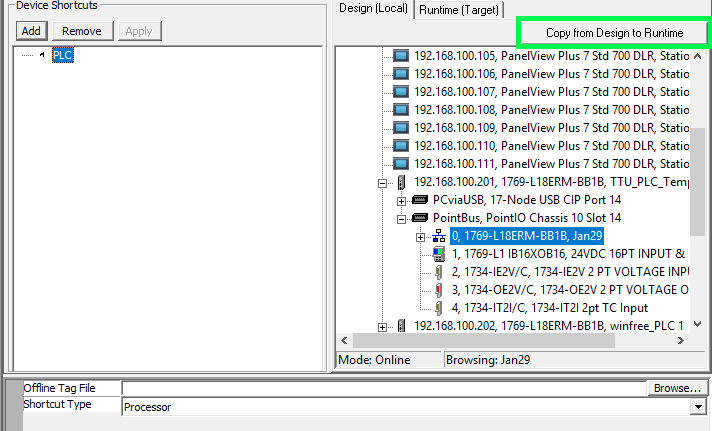
\includegraphics[width=3.2in]{CopyFromDesignToRuntime}}
\caption{Location of copy from design to runtime button}
\label{fig:CopyfromDesignToRuntime}
\end{figure}

The last step to setting up the communication between the PLC and HMI is to accept the communication settings that you have now put in place. To do this click OK in the lower right of the window. Refer to \figureautorefname \ref{fig:FinalizeCommunicationSettings}.

\begin{figure}[h]
\centering
\textbf{Finalize communication setup}\par \medskip
\frame{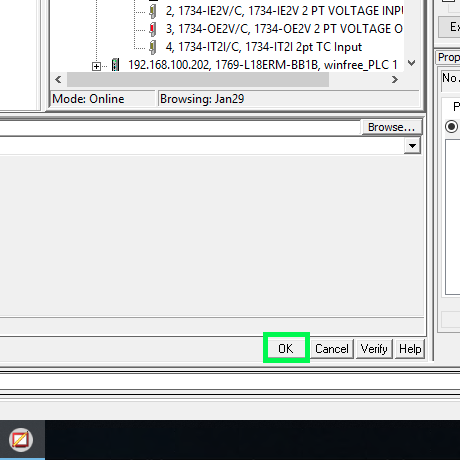
\includegraphics[width=3.2in]{FinalizeCommunicationSettings}}
\caption{Ok to finalize HMI/PLC communication setup}
\label{fig:FinalizeCommunicationSettings}
\end{figure}


\subsection{Create the Runtime Application}

Go to the Application menu and select \textbf{Create Runtime Application}. In the dialog window that appears, \textbf{select save}. This compiles the application into an HMI "runtime". A "Runtime" is what is downloadable to the HMI. 

\subsection{Download the HMI application}

Go to the tools menu and select \textbf{Transfer Utility}. This opens another application which is used to transfer the HMI runtime application to the physical HMI. In the window that appears do the following:

\begin{enumerate}
    \item Click the box with the ellipse next to the source file entry bar
    \item Select the application you created and click open
    \item Check the box beside \textbf{run application at startup}
    \item Check the box beside \textbf{replace communications when transferring the HMI application}
\end{enumerate}

Next you must select the IP address associated with the HMI to which you would like to download the runtime application. The HMI IP address is also associated with your lab seat. Refer to \tableautorefname \ref{Table:HMIIpAddresses} to find the IP address of the HMI associated with your lab seat. 

After identifying the correct HMI IP address, \textbf{highlight the appropriate HMI in the transfer utility window and select download}.

\aside{You may be prompted that an application with this name already exists in the HMI. It is ok to overwrite the existing application.}

\begin{table}[h]
\centering
\caption{HMI IP addresses}
\label{Table:HMIIpAddresses}
\begin{tabular}{c l | c l}
\toprule
Seat \# & IP Address & Seat \# & IP Address\\
\midrule
1 & $192.168.100.101$ & 2 & $192.168.100.102$ \\
3 & $192.168.100.103$ & 4 & $192.168.100.104$ \\
5 & $192.168.100.105$ & 6 & $192.168.100.106$ \\
7 & $192.168.100.107$ & 8 & $192.168.100.108$ \\
9 & $192.168.100.109$ & 10 & $192.168.100.110$ \\
11 & $192.168.100.111$ & 12 & $192.168.100.112$ \\
\bottomrule
\end{tabular}
\end{table}

\subsection{Testing the HMI application}

Once the download completes and the HMI reboots, the application should be running on the HMI screen. There should be a button and display. 

The button has the text "check code". This will check to see if the edits you make to the code in the coming sections is correct. If it is correct, the HMI will tell you that you have correctly written the code. If you hold down the button it will display the word release, instructing you to stop pressing the button.

\aside{For the first several labs we will provide an HMI application that you must download to the HMI. The HMI application will work with code built into the lab PLC file that we provide to notify you if your code is correct and give you feedback.}

\TASignatureSlot


\section{Online ladder program edits}

There are two ways to edit the PLC program. The first is called an online edit and the second is an offline program edit. Online program edits allow the programmer to change the code while the PLC is still in Run mode. An offline PLC program edit requires a download after the edit is complete. Anytime a programmer downloads to the PLC, the PLC is automatically taken out of Run mode and put into Program mode. Typically, after the download completes the programmer is prompted to put the PLC back into Run mode.

\aside{In a laboratory environment it is fine to stop the PLC from executing briefly to perform a download. However, imagine what would happen if the PLC that is used to control the Tennessee Tornado at DollyWood were to be taken out of Run mode in the middle of a ride!}

In this section you will be making an online edit to the program to fix the logical error in the lab 0 program.

\subsection{What's wrong with the logic}

Before you can edit the program, you must figure out what is wrong with the logic. In \figureautorefname \ref{fig:TheCode}, the code is shown. The code is intended to decide if it is Fall based on the month. This doesn't mean that it is deciding if it is Fall based on the current month in the real world, but rather based on which month is "on". 

The add on instruction (AOI) in the upper right hand corner of  \figureautorefname \ref{fig:TheCode} called Lab0\textunderscore IsItFallYet has several attributes associated with it. Some are inputs and some are outputs. Particularly, it has the attributes shown in \tableautorefname \ref{Table:Lab0.1Attributes}.

To access any of these attributes, the dot operator is used. This is why above the contact on the left side of the rung of code in \figureautorefname \ref{fig:TheCode} it says "Lab0.October". Lab0 is the name given to the \textbf{tag} that houses all the memory for the Lab0\textunderscore IsItFallYet
AOI.

\aside{An AOI (add on instruction) is an instruction that someone other than Allen Bradley has created. The AOI requires memory. The way that Allen Bradley allocates memory is in the form of tags. So, there must be a tag associated with each occurrence of an AOI in the code.}

So, if the "Lab0.October" bit (boolean tag) is true (or on, or energized) that would mean that it is October. If the "Lab0.October" bit is on then the normally open contact it is associated with will be energized. Think of this like a light switch. If the "Lab0.October" light switch is on, then electricity will pass through it. 

Keeping with the electrical analogy, now that the switch (referred to as a contact) associated with "Lab0.October" is on (because "Lab0.October" is on), then the voltage on the left hand side of the ladder will pass through to the right hand side of the contact associated with "Lab0.October". This voltage will continue along the rung and be applied to the coil associated with the attribute "Lab0.Its\textunderscore Fall". Energizing the a coil associated with a boolean tag sets the value of the tag to true. \textbf{So, if "Lab0.October" is on, then "Lab0.Its\textunderscore Fall" is also on}.

\aside{The left hand side of an instruction (like the normally open contact associated with "Lab0.October") is called the \rungincondition. The right hand side of an instruction is called the \rungoutcondition. If a normally open contact is on (the boolean value associated with the contact is true), then the \rungoutcondition is set equal to the \rungincondition. However, if the normally open contact is off (the boolean value associated with the contact is false), then the \rungoutcondition is always set to off (or low voltage).}

What about if "Lab0.November" is on but "Lab0.October" is off? The \rungoutcondition for the "Lab0.October" contact is off. However, the \rungincondition applied to the "Lab0.November" is on so the \rungoutcondition is also on. So, a high voltage is still applied to the "Lab0.Its\textunderscore Fall" coil.

\begin{table}[h]
\centering
\caption{Attributes available in Lab0}
\label{Table:Lab0.1Attributes}
\begin{tabular}{c c c}
\toprule
Attribute Name & Data Type & Type\\
\midrule
Jan & Bool & Output \\
Feb &  Bool & Output \\
March &  Bool & Output \\
April & Bool & Output \\
May &  Bool & Output \\
June &  Bool & Output\\
July &  Bool & Output \\
August &  Bool & Output \\
September &  Bool & Output \\
October &  Bool & Output \\
November &  Bool & Output \\
December &  Bool & Output \\
\midrule
Its\textunderscore Fall & Bool & Input\\
\bottomrule
\end{tabular}
\end{table}

\subsubsection{What does the code mean logically}

This rung of code implements a logical OR. If either "Lab0.October" OR "Lab0.November" is true, then "Lab0.Its\textunderscore Fall" is also true. If both "Lab0.October" AND "Lab0.November" are false, then "Lab0.Its\textunderscore Fall" is false.

\subsubsection{What should it be?}

In reality, October and November aren't the only Fall months. September is also a Fall month. So, we need to modify the logic so that if either "Lab0.October" OR "Lab0.November" OR "Lab0.September" is true then "Lab0.Its\textunderscore Fall" is also true. 

\subsection{Let's fix this code}

Now that we have identified the problem with the present code, it is time to fix the problem. To do so we are going to make an online edit to the program.

\subsubsection{Making the rung editable}

To edit a rung of code while the programmer (you) is online, \textbf{right click on the number to the left of the rung and select "Start pending rung edits"}. Two versions of the rung will then be on the screen. The top version will have a column of small letter i's to the left of the rung while the bottom has a column of small letter r's to the left of the rung.

\subsubsection{Adding another OR condition}

We want to add another path for the voltage to flow in the case where "Lab0.September" is true. To do this we must first modify the structure of the rung and then add the instructions.

To modify the structure of the rung, highlight the left side of the rung beside "Lab0.November". This is shown in \figureautorefname \ref{fig:HighlightRung}. The next step, shown in \figureautorefname \ref{fig:AddBranch}, is to add a branch to the rung structure. After the branch is added, it needs to be adjusted to suit our needs. Click and drag the right side of the branch so that it matches what is shown in \figureautorefname \ref{fig:DragTheBranch}.

\begin{figure}[h]
\centering
\textbf{Highlight the rung}\par \medskip
\frame{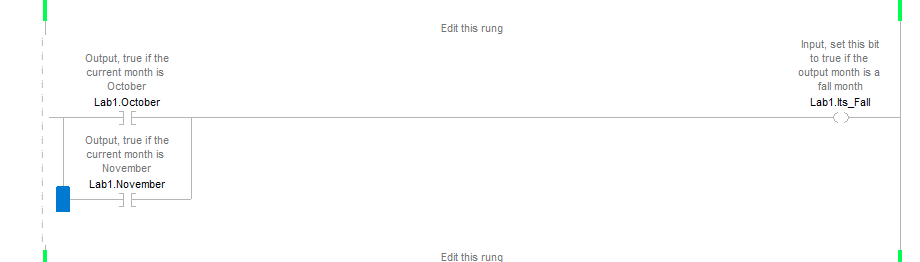
\includegraphics[width=3.2in]{HighlightRung}}
\caption{Highlight the rung that is going to be structurally modified}
\label{fig:HighlightRung}
\end{figure}


\begin{figure}[h]
\centering
\textbf{Add a branch}\par \medskip
\frame{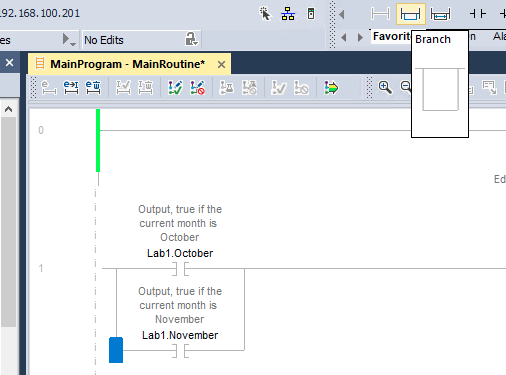
\includegraphics[width=3.2in]{AddBranch}}
\caption{Add a branch to the rung structure}
\label{fig:AddBranch}
\end{figure}


\begin{figure}[h]
\centering
\textbf{Click and drag the branch}\par \medskip
\frame{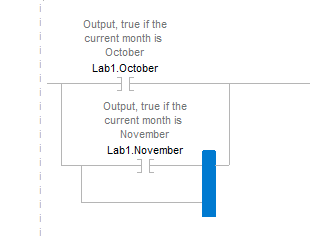
\includegraphics[width=3.2in]{DragTheBranch}}
\caption{Click and drag the branch to suit your needs}
\label{fig:DragTheBranch}
\end{figure}


After the rung is structurally changed to suit our purposes, you must add a contact to adjust the rung logic. Highlight the left hand side of the newly created branch and insert a normally open contact. Refer to \figureautorefname \ref{fig:AddContact}.

\begin{figure}[h]
\centering
\textbf{Add a contact to the branch}\par \medskip
\frame{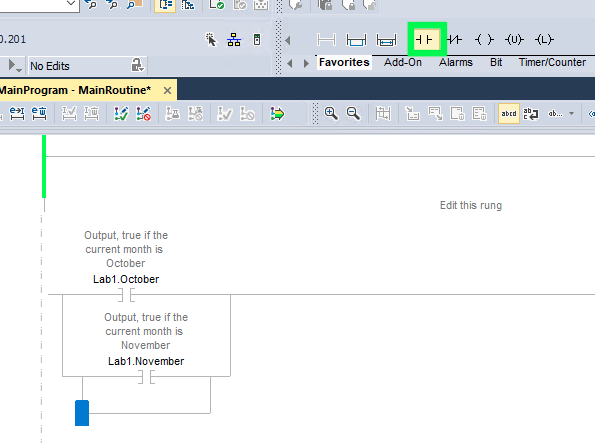
\includegraphics[width=3.2in]{AddContact}}
\caption{Add a contact to the branch}
\label{fig:AddContact}
\end{figure}

At this point there is no tag associated with the contact instruction. So, a question mark appears above the contact. To complete the changes we need to associate this new contact with "Lab0.September". To do this, select the question mark above the contact and type "Lab0.September" without the quotation marks. Press enter when it is fully typed.

\subsubsection{Submitting online edits}

The last step to completing our online edit is to finalize all the edits in the program. To finalize the edits click the button shown in \figureautorefname \ref{fig:FinalizeEdits}. A dialog window will appear asking you to confirm that you wish to finalize the edits. Select yes. If your code did not have any errors, then the code is finalized and is now running in the PLC.

\begin{figure}[h]
\centering
\textbf{Finalize all edits in program}\par \medskip
\frame{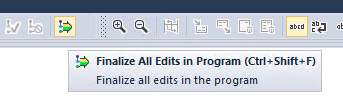
\includegraphics[width=3.2in]{FinalizeEdits}}
\caption{Finalize the online program edits}
\label{fig:FinalizeEdits}
\end{figure}

\subsection{Is it Fall yet?}

Now, press the check code button on the HMI. If you edited the code correctly then your HMI will say so. 

\TASignatureSlot


\section{Offline ladder program edits}

Another way to edit the code, as stated previously, is to take the program offline. While the code is offline, all rungs (in general) are editable. This is often convenient if you have several rungs to edit. However, you will have to perform a download after making offline changes to a program.

In this section you will make an offline edit to the program and download the edited code.

\subsection{How do you know that it is Fall?}

First, let's consider a logical question. How does one know that it is Fall based on the month? Certainly we have found one answer to this question. But is there another way? 

The solution we have used thus far is to check if it is October OR November OR September. If any of these is true then it is also true that it is Fall.

Instead of using a logical OR we can also use the logical AND to infer the state of Fall. The logic goes like this: if it is \textit{not} January AND \textit{not} February AND \textit{not} March AND \textit{not} April AND \textit{not} May AND \textit{not} June AND \textit{not} July AND \textit{not} August AND \textit{not} December, then it must be Fall. 

\subsection{Let's code it}

In order to write this into code, you will have to make use of the normally closed contact (XIO). The normally closed contact will allow the voltage to pass if the boolean tag associated with the normally closed contact is false. This allows us to code \textit{not} January and so forth.

Structurally, the conditions won't be in branches that pass around each other. Rather, each of the normally closed contacts will be placed in series so that the only way for voltage to get to the coil associated with "Lab0.Its\textunderscore Fall" is for the boolean attributes associated with all non-Fall months to be false.

\aside{If a normally closed contact is on (the boolean value associated with the contact is true), then the \rungoutcondition is set to false. However, if the normally closed contact is off (the boolean value associated with the contact is false), then the \rungoutcondition is always set equal to the \rungincondition.}

\aside{XIO and XIC are the actual names of the Allen Bradley normally closed and normally open contacts respectively. The acronym stands for "examine if open" and "examine if closed".\\
--Normally closed means that the normal (not energized) state is closed. This would be like a light switch that allowed current to flow when it was off but stopped the flow of current when the switch was in the on position (a backwards light switch). This is the same as "examine if open".\\
--Normally open means that the normal (not energized) state is open. This would be like a light switch that allowed current to flow when it was on but stopped the flow of current when the switch was in the off position (a typical light switch). This is the same as "examine if closed".}

\subsubsection{Go Offline}

To set the PLC to offline, \textbf{select go offline} under the communications menu.

\subsubsection{Edit the rung - Delete the conditions}

Edit the rung appropriately so that it looks like the one shown in \figureautorefname \ref{fig:NotLogic}.


\begin{figure}[h]
\centering
\textbf{AND based logical approach}\par \medskip
\frame{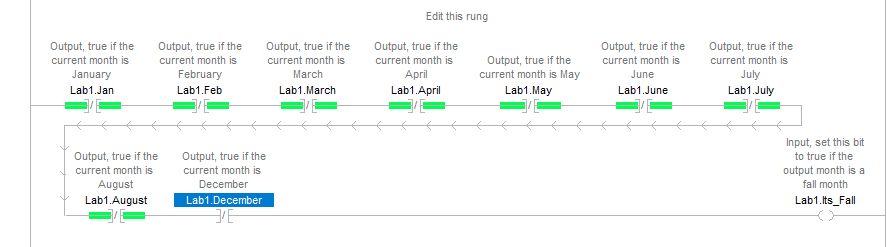
\includegraphics[width=3.2in]{NotLogic}}
\caption{AND based logical approach to deciding it is Fall}
\label{fig:NotLogic}
\end{figure}

\subsubsection{Download}

Download the code to the PLC. If you need guidance on the process, refer to \sectionautorefname \ref{subsection:DownloadPLC}.

\subsubsection{Go Online}

Go online. If you need guidance on the process, refer to \sectionautorefname \ref{subsection:GoOnline}.

\subsection{Is it Fall yet?}

Again press the button on the HMI. If your new logic is correct then HMI will display the same message you saw previously when you fixed the logic used to decide if it is Fall.

\TASignatureSlot


\section{Toggle a bit}

Sometimes it is helpful to be able to toggle a bit from off (false) to on (true) as well as vice versa. Specifically, this is helpful when you want to test a logical circuit under certain conditions.

\subsection{Toggle December}

Allen Bradley provides a convenient keyboard shortcut to toggle a bit. To demonstrate this, highlight the normally closed contact associated with "Lab0.December". With it highlighted, hold the control key and press the T key (ctrl+T). This will change the boolean value of "Lab0.December".

Now, highlight the coil associated with "Lab0.Its\textunderscore Fall" and use the toggle keyboard shortcut.

Why do you think that it doesn't appear to work?

\aside{The PLC is executing the code continuously while in Run mode. This execution happens in under a few milliseconds on an Allen Bradley PLC. So, if you attempt to toggle the state of a boolean tag which is being "driven" (another term for being associated with a coil), then the PLC quickly overwrites the result of your toggle command with the logical result from the output coil.}

Demonstrate your ability to use the toggle shortcut to the TA.

\TASignatureSlot